% Ref: https://www.overleaf.com/latex/templates/emory-poster-template/skpfmpxjnqdh

\documentclass[25pt, a0paper, landscape, margin=10mm, innermargin=15mm, blockverticalspace=10mm, subcolspace=7mm, dvipsnames]{tikzposter} % you need to leave in dvipsnames or else it undoes the orange edge colour??

\usepackage[T1]{fontenc}
\usepackage{helvet}
%\usepackage[utf8]{inputenc}
\usepackage{amsmath}
\usepackage{amsfonts}
\usepackage{amsthm}
\usepackage{amssymb}
\usepackage{mathrsfs}
\usepackage{graphicx}
\usepackage{adjustbox}
\usepackage{enumitem}
\usepackage[backend=bibtex,style=numeric, citestyle=ieee]{biblatex}
\usepackage{xpatch}
\usepackage{xcolor}
\usepackage{multicol}
\usepackage{lipsum}
\usepackage{setspace}

\setlength{\columnsep}{2.5cm}
\setlength{\columnseprule}{1mm}
\pagecolor{Dandelion}

% Ref: https://latex-cookbook.net/poster/
\renewcommand*{\familydefault}{\sfdefault}% Let's have a sans serif font

% set theme parameters
\tikzposterlatexaffectionproofoff
\usepackage{anyfontsize}
\usetheme{Default}
\usebackgroundstyle{Default}
\definecolor{epccnavy}{HTML}{1D2A3D}
\definecolor{universityred}{HTML}{D50032}
\colorlet{backgroundcolor}{white} % <<< this makes bg white
\colorlet{framecolor}{epccnavy}%Dandelion}
\colorlet{titlefgcolor}{epccnavy}
\colorlet{blocktitlebgcolor}{epccnavy}
\colorlet{blocktitlefgcolor}{white}
\colorlet{blockframecolor}{epccnavy}

% \definetitlestyle{sampletitle}{
%     width=800mm, 
%     roundedcorners=20, 
%     linewidth=10pt, 
%     innersep=10pt,
%     titletotopverticalspace=15mm, titletoblockverticalspace=25mm 
% }{
% \begin{scope}[line width=\titlelinewidth, rounded corners=\titleroundedcorners]
% \draw[color=blocktitlebgcolor, fill=titlebgcolor]
% (\titleposleft,\titleposbottom) rectangle (\titleposright,\titlepostop);
% \end{scope}
% }
% \usetitlestyle[]{sampletitle}


% Ref: https://tex.stackexchange.com/questions/309713/modify-font-style-in-title-of-tikzposter
\settitle{ \centering
\vbox{
    \begin{spacing}{1.2}
    %\@titlegraphic \\[\TP@titlegraphictotitledistance] \centering
    \color{titlefgcolor} {\sffamily \bfseries \huge  \textsc{\@title} \par}
    \vspace*{0.75em}
    \color{universityred} {\sffamily \bfseries \huge \subtitle}   
    %\vspace*{0.2em}
    \begin{flushleft}
    {\color{titlefgcolor} {\sffamily \huge \@author}
    \hspace{0.4em}
    {\sffamily \LARGE \@institute \par}}
    \end{flushleft}
    \end{spacing}
}
}
\makeatother

% Ref: https://tex.stackexchange.com/questions/180234/how-can-i-make-my-title-wrap-in-a-tikzposter
\makeatletter
\def\title#1{\gdef\@title{\scalebox{\TP@titletextscale}{%
			\begin{minipage}[t]{\linewidth}
				%\centering
				#1
			\par
				\vspace{0.5em}
			\end{minipage}%
}}}
\makeatother

% Ref: https://tex.stackexchange.com/questions/263563/add-logos-beyond-the-title-tikzposter
%\title{\parbox{\linewidth}{Do Research Software Developer Personas Exist? Are *YOU* an RS-10X? \\ Identifying Distinct Developer/Repository Interaction Types by Mining GitHub Data}}
\title{\parbox{\linewidth}{\fontseries{bx}\selectfont {\fontsize{78}{78}\selectfont {Identifying Research Software Developer Personas Could Create Better Research Software Developers} }}}
\newcommand{\subtitle}{Are YOU an RS-10X? Mining GitHub to Describe Developer/Repository Interaction Types}
\author{\textbf{Felicity `Flic' Anderson\textsuperscript{$\dagger$}, Dr. Julien Sindt\textsuperscript{$\dagger$} \& Prof. Neil Chue Hong\textsuperscript{$\dagger$}}}
\institute{\textsuperscript{$\dagger$}EPCC, University of Edinburgh}
%\titlegraphic{
\includegraphics{epcclogo.png}}

\makeatletter
\newcommand\insertlogoi[2][]{\def\@insertlogoi{\includegraphics[#1]{#2}}}
%\newcommand\insertlogoi[2][]{\def\@insertlogoi{\hspace*{0.5in}\includegraphics[#1]{#2}}}
\newcommand\insertlogoii[2][]{\def\@insertlogoii{\includegraphics[#1]{#2}}}
%\newcommand\insertlogoii[2][]{\def\@insertlogoii{\hspace*{-7.5in}\includegraphics[#1]{#2}}}
%\newcommand\insertlogoiii[2][]{\def\@insertlogoiii{\includegraphics[#1]{#2}}}
\newlength\LogoSep
\setlength\LogoSep{0pt}

\insertlogoi[width=14cm]{informaticsUoE.png}
\insertlogoii[width=15cm]{epcclogo.png}
%\insertlogoii[width=15cm]{EpccANDEmailQRsidebyside.png}

\renewcommand\maketitle[1][width=800mm, linewidth=6pt]{  % #1 keys
	\normalsize
	\setkeys{title}{#1}
	% Title dummy to get title height
	\node[transparent,inner sep=\TP@titleinnersep, line width=\TP@titlelinewidth, anchor=north, minimum width=\TP@visibletextwidth-2\TP@titleinnersep]
	(TP@title) at ($(0, 0.5\textheight-\TP@titletotopverticalspace)$) {\parbox{\TP@titlewidth-2\TP@titleinnersep}{\TP@maketitle}};
	\draw let \p1 = ($(TP@title.north)-(TP@title.south)$) in node {
		\setlength{\TP@titleheight}{\y1}
		\setlength{\titleheight}{\y1}
		\global\TP@titleheight=\TP@titleheight
		\global\titleheight=\titleheight
	};
	
	% Compute title position
	\setlength{\titleposleft}{-0.5\titlewidth}
	\setlength{\titleposright}{\titleposleft+\titlewidth}
	\setlength{\titlepostop}{0.5\textheight-\TP@titletotopverticalspace}
	\setlength{\titleposbottom}{\titlepostop-\titleheight}
	
	% Title style (background)
	\TP@titlestyle
	
	% Title node
	\node[inner sep=\TP@titleinnersep, line width=\TP@titlelinewidth, anchor=north, minimum width=\TP@visibletextwidth-2\TP@titleinnersep]
	at (0,0.5\textheight-\TP@titletotopverticalspace)
	(title)
	{\parbox{\TP@titlewidth-2\TP@titleinnersep}{\TP@maketitle}};
	
	\node[inner sep=0pt,anchor=west] 
	at ([xshift=-\LogoSep]title.west)
	{\@insertlogoi};
	
	\node[inner sep=0pt,anchor=east] 
	at ([xshift=\LogoSep]title.east)
	{\@insertlogoii};
	
	% Settings for blocks
	\normalsize
	\setlength{\TP@blocktop}{\titleposbottom-\TP@titletoblockverticalspace}
}
\makeatother

\onehalfspacing
% begin document
\begin{document}
%\useblockstyle{Basic}
\maketitle
\begin{columns}
\column{.5}

\block[linewidth=5pt]{0: Identifying the Habits of Highly Effective Developers}{
    \vspace{0.4em}
    {\fontsize{42}{42}\selectfont 
    %\vspace{1em}
    \textbf{This pilot study attempts to identify `superstar developers' within 10 larger RS repositories by exploring assignment and contributions data.}
    \vspace{1em}
    \begin{itemize}
    \setlength{\itemindent}{0.5em}
    \setlength\itemsep{0.2em}
        %\item \textbf{Mining Research Software (RS) repository data can help understand RS development practices.}  
        \item Assignment to GitHub features Issue Tickets (ITx) and Pull Requests (PRs) correlate with commit contributions.
        \item Individually limited metrics can be combined to give better picture of development responsibilities or activity.
        \item \textbf{Can this approach locate distinct clusters of behaviours and define and describe RS developer personas? Can they predict effectiveness?} 
    \end{itemize}
    %\vspace{1em}
    }
    %{\fontsize{45}{45}\selectfont
    %This pilot study attempts to identify `superstar developers' within 10 larger RS repositories by exploring assignment and contributions data.  
    %\vspace{1em}
    %}        % via https://tex.stackexchange.com/a/499070
} 
\block[linewidth=5pt]{1: Mining RS Repository Data To Understand Dev/Repo Interactions}{
    \begin{multicols}{2}
    %\vspace{1em}
    {\fontsize{40}{40}\selectfont 
        %https://\textbf{zenodo}.org/api/records API was queried for software records with a DOI (common in published research software); 
        % records were selected with a `github.com' URL. These were presumed to be RS repositories. 
        
        %These repositories were mined via \textbf{GitHub REST API} to gather repository statistics (xxxxxxx, yyyyyyyy, zzzzzzzz), contributor data (xxxxxxx, yyyyyyyy, zzzzzzzz), and issue ticket data and pull request data (xxxxxxx, yyyyyyyy, zzzzzzzz).  

        % inclusion/exclusion criteria... languages, size, age, etc 

        % table of stats for total repo dataset N=1823 number of devs; average commits; average repo age; average number of issue tickets / PRs; 


        %This larger dataset was subset to select repositories with larger numbers of developer contributors: 

        % table of stats for subset big10 dataset N=10: number of devs; average commits; average repo age; average number of issue tickets / PRs; 

        % PLOT: issue ticket and PR usage yes vs no
        % UPGRADE: split yes into assigned vs unassigned 
        
        \begin{tikzfigure}
            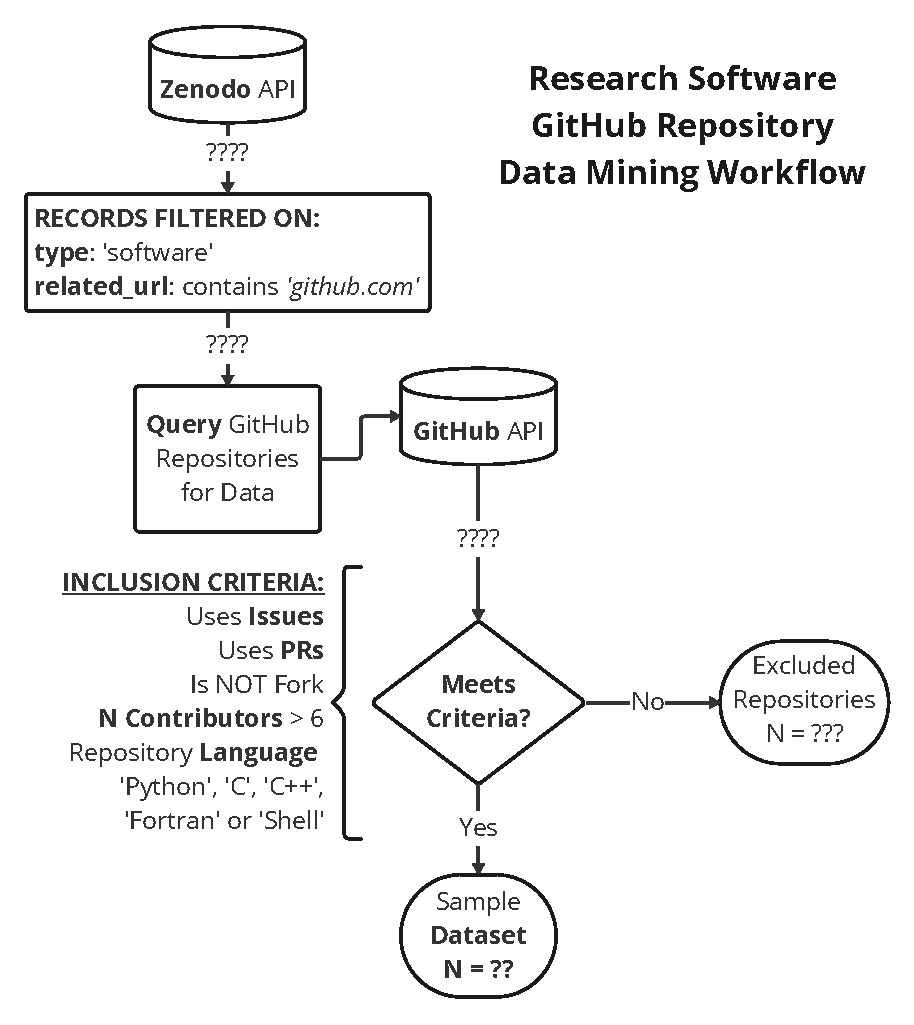
\includegraphics[height=270mm]{Figures/epccposter - DataMiningWorkflow.pdf}
        \end{tikzfigure}

        Research Software is any software used to generate research, across academic fields. 
        % Dev Personas in OSS; SE  
        % What do we know about how RSEs interact with their repos?  Repo usage at all %?  
        % Data Mining background as a method 
        \vspace{1em}
        
        Quisque varius id dolor sed congue. Proin mollis lorem et tellus sodales, sit amet hendrerit urna vulputate. Cras maximus, dolor non laoreet vulputate, nisl nisl cursus ex.
        \begin{tikzfigure}[]
        %\setlength{\belowcaptionskip}{-8pt}
            \includegraphics[width=0.96\linewidth]{Figures/bars_usage.png}
        \end{tikzfigure}
        }
        \end{multicols}
        }
\block[linewidth=3pt]{}{
    \textbf{Contact: Felicity.Anderson@ed.ac.uk} \hspace{0.5em} 
    \textbf{Acknowledgements:} Funded by EPSRC funding details details details.
    \textbf{References:} Lorem ipsum dolor sit amet, consectetur adipiscing elit. Morbi condimentum ipsum tortor, sit amet elementum eros auctor sed.
    }

\column{.5}
\block[linewidth=5pt]{2: More Responsibility = More Action?}{
    \begin{multicols}{2}
    
    {\fontsize{40}{40}\selectfont 
    \textbf{Context \& Demographics} \newline 
    %Around a third of repositories use Issues and PRs. 
    TEXT ABOUT CONTENT AND DEMOGRAPHICS ETC ETC ETC 
    % RS repos with github.coms vs not. 
    % repo age 
    % repo size (N commits) 
    % dev team size (N Devs) 
    % repo recent activity  
    % languages 
    % Repos with issues and prs vs Not using.
    % numbers of issues and PRs
    \vspace*{0.4em} 
    \par
    
    \textbf{Assignment Practices} \newline  
    NNN of NNN items in NNN repositories were assigned to 1+ developers.   
    % BEWARE! _s need to be escaped for usage. 
    %\vspace*{0.1em}
    % TABLE OF ASSIGNMENT CATEGORIES PERCENTAGE
    \begin{center}
    \begin{tabular}{ l c c c} 
     %\hline
     \textbf{Assignment}\\ \textbf{Category} & \textbf{Devs (\%)} \\
     %\hline
     BOTH & 00 \\ 
     %\hline
     ISSUES\_ONLY & 00 \\
     %\hline
     PRs\_ONLY & 00 \\
     %\hline
     NEITHER & 00 \\ 
     %\hline
    \end{tabular}
    \end{center}
    %\vspace*{0.1em}
    Assignment types were categorised as \textit{being assigned to 1+ Issue and/or 1+ PR}
    \vspace*{0.4em} 
    \par
    
   
    \textbf{Commit Contributions} \newline 
    % Contribution numbers overall.    
    % Commits per dev contribution as proportion of their repo total  
    % Commits per dev average across 10 repos by assignment category  
    Commit numbers positively correlate with number of items assigned. \textit{Activity and responsibility proxies seem to correlate.}
    \vspace*{0.4em} 
    \par
    
    \textbf{Developer Interaction Types} \newline 
        \begin{tikzfigure}[]
        %\setlength{\belowcaptionskip}{-8pt}
            \includegraphics[width=0.95\linewidth]{Figures/correlations-lmplot.png}
        \end{tikzfigure}
    %High impact grouping vs low impact grouping
    Developers assigned to 'BOTH' item types have almost 10\% higher commit numbers than all other assignment groups. 
    These might make up a 'highly interactive' type. 
    Differences between Assignment Category groupings lay RS Developer Personas groundwork.
    \par
    }
    \end{multicols}
}
\block[linewidth=5pt]{3: Using RS Developer Personas in Future Work}{
    \vspace{1em}
    {\fontsize{40}{40}\selectfont 
    

    %\textbf{Findings} \newline 
    Larger team sizes more likely to use Issues and PRs. WHY? They are a communication tool. [CITATION NEEDED!] 
    Assignment is rare within wider RS population, but a feature of high-interaction repositories.
    % WHY?
    [CITATION NEEDED!]     
    \newline
    \vspace*{0.4em} 
    \textbf{Non-random selection} of larger repositories using Zenodo \& GitHub services means users already follow some 'best practice'.  
    'Accepted practices' within repositories may restrict development options, while RS projects can be hard to compare in terms of development style, RS goals, or effort intensity.
    \textbf{Projects change} over time, practices may change to reflect this - how can we capture 'typical' behaviour?  
    This work \textbf{does not establish causation} between assignment and commit numbers. 
    }
}
\end{columns}
\end{document}